


%%%%%%%%%%%%%%%%%%%%%%%%%%%%%%%%%%%%%%%%%%%%%%%%%%%%%%%%%%%%%%%%%%%%%%%%
\section{Agentes Racionais}


\begin{frame}

\begin{center}
{\huge Capítulo 2 -- Agentes Racionais}
\end{center}

\end{frame}




%--------------------------------------------
\begin{frame} [allowframebreaks=0.9]

    \frametitle{O que é um Agente?}

\begin{block}{Qualquer entidade (humana ou artificial) que:}
  
  \begin{itemize}
    \item está \textbf{imersa} ou \textbf{situada} em um ambiente (físico, virtual/simulado) 
    \item \textbf{percebe} ou \textbf{sente} seu ambiente através de sensores (ex. câmeras, microfone, teclado, finger, ...)
    \item \textbf{age} sobre ele através de atuadores (ex. vídeo, auto-falante, impressora, braços, ftp, ...)
    \item \textbf{possui objetivos} próprios:
explícitos ou implícitos
    \item \textbf{escolhe} suas ações em função das suas percepções para atingir seus objetivos
  
  \end{itemize}
  
\end{block}

\end{frame}
%--------------------------------------------


%--------------------------------------------
\begin{frame} [allowframebreaks=0.9]

    \frametitle{Agente Situado x Não-Situado}

\begin{block}{uma figura aqui }
  
  
\end{block}

\end{frame}
%--------------------------------------------


%--------------------------------------------
\begin{frame} [allowframebreaks=0.9]

    \frametitle{O que é um Agente Racional?}

\begin{block}{}
  
 \begin{itemize}
      \item Agente Racional 
 \begin{itemize}
        \item faz a melhor coisa possível
        \item segue o princípio da racionalidade:\\ 
dada uma seqüência perceptiva, o agente escolhe, segundo seus conhecimentos, as ações que melhor satisfazem seu objetivo
      \end{itemize}

\begin{itemize}
  \item Limitações de:\\
  sensores\\
  atuadores\\
  raciocinador (conhecimento, tempo, etc.)
\end{itemize}

    \end{itemize}
  
\end{block}

\end{frame}
%--------------------------------------------



%--------------------------------------------
\begin{frame} [allowframebreaks=0.9]

    \frametitle{Outras propriedades freqüentemente 
associadas aos Agentes}


  
    \begin{itemize}
      \item Autonomia:\\
raciocínio, comportamento guiado por objetivos ou \\
reatividade

\begin{itemize}
  \item Requer máquina de inferência e base de conhecimento
  \item Essencial em sistemas especialistas, controle, robótica, jogos, agentes na internet ...
\end{itemize}
      
    \item Adaptabilidade \& aprendizagem
             
    \begin{itemize}
             
    \item Capacidade de adaptação a situações novas, para as quais não foi fornecido todo o      conhecimento necessário com antecedência 

     \item Duas implementações: sistema com  
           aprendizagem 
           e/ou programação declarativa
  
     \item Essencial em agentes na internet, interfaces amigáveis ...
   
    \end{itemize}
             
             
    \item Comunicação \& Cooperação (Sociabilidade
         \begin{itemize}
          \item  Protocolos padrões de comunicação, cooperação, negociação
          \item  Raciocínio autônomo sobre crenças e confiabilidade
          \item   Arquiteturas de interação social entre agentes
                      
         \end{itemize}
         
                
    \item Personalidade
    
    \begin{itemize}
      \item IA + modelagem de atitudes e emoções
      \item Essencial em entretenimento digital, realidade virtual, interfaces amigáveis ... 
    \end{itemize}
    
    \item Continuidade temporal (persistência)
    \begin{itemize}
      \item Requer interface com sistema operacional e banco de dados
    \item Essencial em filtragem, monitoramento, controle, ...
    \end{itemize}
    
    
 \item Mobilidade (caso internet)
  \begin{itemize}
     \item Requer itens como:
     \begin{enumerate}
       \item Interface com rede
       \item Protocolos de segurança
       \item Suporte a código móvel
     \end{enumerate}

    \item Essencial em agentes de exploração da internet, ...
         
     \end{itemize}      
                  
    \end{itemize}
 
\end{frame}
%--------------------------------------------




%--------------------------------------------
\begin{frame} [allowframebreaks=0.9]

    \frametitle{O que é um Agente?}

\begin{block}{Qualquer entidade (humana ou artificial) que:}
  
    \begin{itemize}
      \item 
      \pause
          \item 
              \pause
              \item 
                  \pause
                  \item 
    \end{itemize}
  
\end{block}

\end{frame}
%--------------------------------------------



\begin{frame}

    \frametitle{Características aos SMAs}
    \begin{itemize}
    \pause
      \item 
\pause
      \item cap 2
    
    \end{itemize}
\end{frame}

\subsection{Tipos de Agentes}
\begin{frame}

Os agentes podem ser de dois tipos:
\begin{description}

 \item[Agentes Reativos (ou reflexivos):] geralmente são agentes simples, escolhem suas ações baseados exclusivamente nas percepções que têm do ambiente. Normalmente possui representação do conhecimento implícito  no código, por não  possuirem
  memória, não tem histórico dos fatos  e das ações que executou.

  \item[Agentes Cognitivos:]  têm uma representação simbólica explícita do seu ambiente, no qual eles podem argumentar e predizer eventos futuros. São dirigidos por intenções, isto é, por metas explícitas que conduzem seu comportamento e os tornam capazes de escolher entre possíveis ações. 
  Engloba as características: percepção, ação, comunicação, representação, 
  motivação, deliberação, raciocínio e aprendizagem. 

\end{description}

\end{frame}


\subsection{Agentes Racionais}

\begin{frame}

  \frametitle{Agente em seu ambiente}
    
\begin{figure}[!ht]
  \centering
  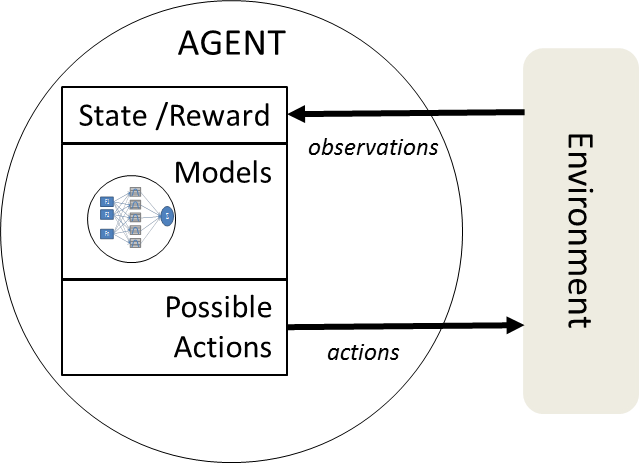
\includegraphics[height =.6\textheight,width=.7\textwidth]{figuras/agente_ambiente_ciclo.png}
  \caption{Ciclo do agente}
%\label{ag_01}
\end{figure}
    
\end{frame}



\begin{frame}

  \frametitle{Arquitetura clássica de um agente reflexivo}
    
\begin{figure}[!ht]
\centering
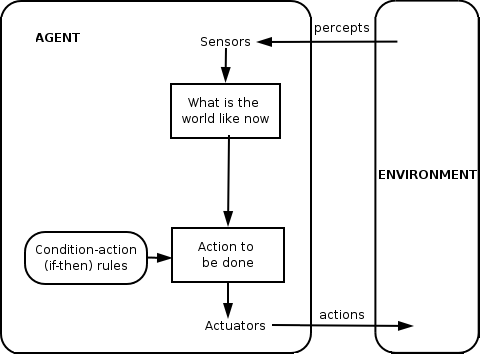
\includegraphics[width=.6\textwidth]{figuras/agent-reflexivo.png}
\caption{Arquitetura clássica}
\label{ag_01}
\end{figure}
    
\end{frame}


\begin{frame}

  \frametitle{Arquitetura clássica de um agente que \textit{aprende} -- desejável}
    
\begin{figure}[!ht]
\centering
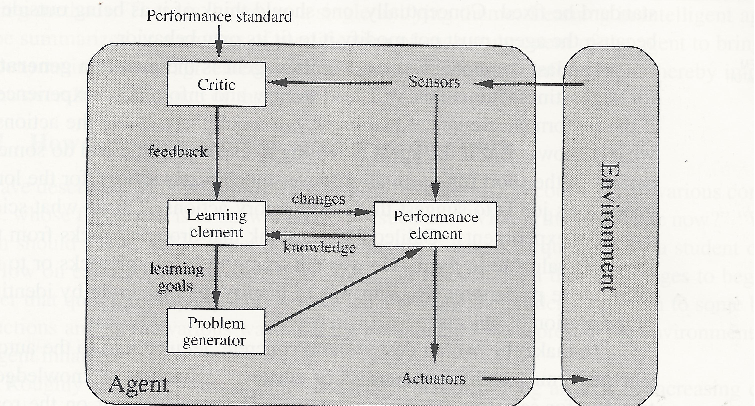
\includegraphics[height =.6\textheight,width=.7\textwidth]{figuras/agent-learning.pdf}
\caption{Arquitetura agente com aprendizagem}
\label{ag_02}
\end{figure}
    
\end{frame}
